% defer/seqlock.tex

\section{Sequence Locks}
\label{sec:defer:Sequence Locks}

\begin{figure}[tb]
\begin{center}
\resizebox{3in}{!}{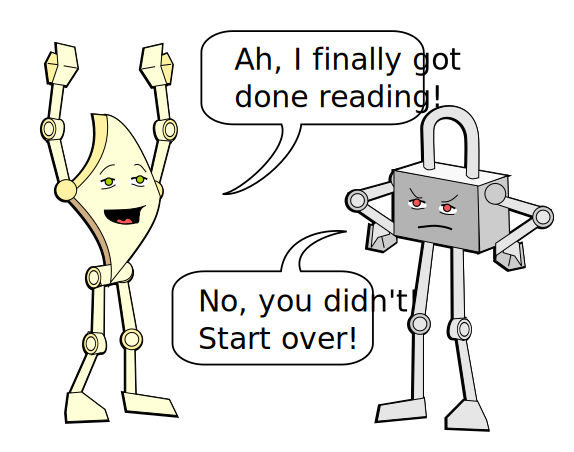
\includegraphics{cartoons/r-2014-Start-over}}
\end{center}
\caption{Reader And Uncooperative Sequence Lock}
\label{fig:defer:Reader And Uncooperative Sequence Lock}
\end{figure}

시퀀스 락은 읽기를 하는 쓰레드들에게 일관적인 상태로 보여야만 하는 읽기가
대부분 이루어지는 데이터를 위해 리눅스 커널에서 사용됩니다.
하지만, reader-writer 락킹과 달리, 읽기를 하는 쓰레드들은 쓰기를 하는
쓰레드들을 배타시키지 않습니다.
대신에, 해저드 포인터처럼, 시퀀스 락들은 읽기를 하는 쓰레드들이 동시에 수행중인
쓰기를 하는 쓰레드들로부터의 동작이 탐지되면 오퍼레이션을 \emph{재시도} 하도록
강제합니다.
Figure~\ref{fig:defer:Reader And Uncooperative Sequence Lock} 에 보여지는
것처럼, 읽기를 하는 쓰레드들이 재시도를 하는 경우는 매우 드문 경우일 수 있도록
시퀀스 락을 사용해 코드를 설계하는 것이 중요합니다.
\iffalse

Sequence locks are used in the Linux kernel for read-mostly data that
must be seen in a consistent state by readers.
However, unlike reader-writer locking, readers do not exclude writers.
Instead, like hazard pointers, sequence locks force readers to
\emph{retry} an operation if they detect activity from a concurrent writer.
As can be seen from
Figure~\ref{fig:defer:Reader And Uncooperative Sequence Lock},
it is important to design code using sequence locks so that readers
very rarely need to retry.
\fi

\QuickQuiz{}
	왜 이 시퀀스 락에 대한 토론은 Chapter~\ref{chp:Locking} 에서,
	\emph{locking} 의 하나로써 다루어지지 않았던 거죠?
	\iffalse

	Why isn't this sequence-lock discussion in Chapter~\ref{chp:Locking},
	you know, the one on \emph{locking}?
	\fi
\QuickQuizAnswer{
	시퀀스 락 메커니즘은 실제로는 시퀀스 카운트와 락킹이라는 두개의 별개의
	동기화 메커니즘들의 조합입니다.
	사실, 시퀀스 카운트 메커니즘은 리눅스 커널에서
	\co{write_seqcount_begin()} 과 \co{write_seqcount_end()} 기능들을
	사용해 별개로 사용될 수도 있습니다.
	\iffalse

	The sequence-lock mechanism is really a combination of two
	separate synchronization mechanisms, sequence counts and
	locking.
	In fact, the sequence-count mechanism is available separately
	in the Linux kernel via the
	\co{write_seqcount_begin()} and \co{write_seqcount_end()}
	primitives.
	\fi

	하지만, 조합된 \co{write_seqlock()} 과 \co{write_sequnlock()} 기능들은
	리눅스 커널에서 훨씬 많이 사용됩니다.
	더 중요한건, 더 많은 사람들이 ``시퀀스 카운트'' 라고 말하는 것보다는
	``시퀀스 락'' 이라고 말하는 걸 더 쉽게 이해할 것이라는 점입니다.

	그래서 이 섹션은 사람들이 제목으로부터 이게 뭐에 대한 것인지를 이해할
	수 있도록 ``Sequence Locks'' 라고 이름지어졌고, ``Deferred Processing''
	으로 표현한 이유는 (1) ``시퀀스 락'' 에서 ``시퀀스 카운트'' 의 강조를
	위함과 (2) ``시퀀스 락'' 은 단순한 락보다는 더 많은 의미를 갖기
	때문입니다.
	\iffalse

	However, the combined \co{write_seqlock()} and
	\co{write_sequnlock()} primitives are used much more heavily
	in the Linux kernel.
	More importantly, many more people will understand what you
	mean if you say ``sequence lock'' than if you say
	``sequence count''.

	So this section is entitled ``Sequence Locks'' so that people
	will understand what it is about just from the title, and
	it appears in the ``Deferred Processing'' because (1) of the
	emphasis on the ``sequence count'' aspect of ``sequence locks''
	and (2) because a ``sequence lock'' is much more than merely
	a lock.
	\fi
} \QuickQuizEnd

\begin{listing}[bp]
{ \scriptsize
\begin{verbbox}
  1 do {
  2   seq = read_seqbegin(&test_seqlock);
  3   /* read-side access. */
  4 } while (read_seqretry(&test_seqlock, seq));
\end{verbbox}
}
\centering
\theverbbox
\caption{Sequence-Locking Reader}
\label{lst:defer:Sequence-Locking Reader}
\end{listing}

\begin{listing}[bp]
{ \scriptsize
\begin{verbbox}
  1 write_seqlock(&test_seqlock);
  2 /* Update */
  3 write_sequnlock(&test_seqlock);
\end{verbbox}
}
\centering
\theverbbox
\caption{Sequence-Locking Writer}
\label{lst:defer:Sequence-Locking Writer}
\end{listing}

시퀀스 락킹에서의 핵심 컴포넌트는 시퀀스 넘버로, 이 수는 업데이트를 하는
쓰레드가 존재하지 않는다면 짝수를 가지고 진행 중인 업데이트가 있다면 홀수를
갖습니다.
읽기를 하는 쓰레드들은 각각의 액세스 전과 후로 이 값을 스냅샷을 뜰 수 있습니다.
만약 두 스냅샷 중 하나라도 홀수이거나, 두 스냅샷이 서로 다르다면, 동시에
업데이트가 있었다는 것이고, 따라서 읽기를 한 쓰레드는 해당 액세스의 결과를
버리고 다시 읽기를 시도해야 합니다.
시퀀스 락으로 보호되는 데이터에 대해 읽기를 하기 위해서는 \co{read_seqbegin()}
과 \co{read_seqretry()} 함수들이 Listing~\ref{lst:defer:Sequence-Locking Reader}
와 같이 사용되어야 합니다.
쓰기를 하는 쓰레드들은 각가의 업데이트 전과 후에 그 값을 증가시켜야 하는데,
한번에 하나의 읽기 쓰레드의 수행만이 허가되어 있습니다.
쓰기를 하는 쓰레드들은 시퀀스 락으로 보호되는 데이터를 업데이트 하기 위해서는
\co{write_seqlock()} 과 \co{write_sequnlock()} 함수를
Listing~\ref{lst:defer:Sequence-Locking Writer} 에 보여진 것처럼 사용합니다.
\iffalse

The key component of sequence locking is the sequence number, which has
an even value in the absence of updaters and an odd value if there
is an update in progress.
Readers can then snapshot the value before and after each access.
If either snapshot has an odd value, or if the two snapshots differ,
there has been a concurrent update, and the reader must discard
the results of the access and then retry it.
Readers therefore use the \co{read_seqbegin()} and \co{read_seqretry()}
functions shown in Listing~\ref{lst:defer:Sequence-Locking Reader}
when accessing data protected by a sequence lock.
Writers must increment the value before and after each update,
and only one writer is permitted at a given time.
Writers therefore use the \co{write_seqlock()} and \co{write_sequnlock()}
functions shown in Listing~\ref{lst:defer:Sequence-Locking Writer}
when updating data protected by a sequence lock.
\fi

따라서 시퀀스 락으로 보호되는 데이터는 상당히 많은 수의 동시에 수행되는 읽기를
하는 쓰레드들을 가질 수 있습니다만, 쓰기를 하는 쓰레드는 한번에 하나씩만
가능합니다.
시퀀스 락킹은 시간 계측에 사용되는 값의 측정을 보호하기 위해 사용됩니다.
시퀀스 락킹은 또한 동시적인 이름 바꾸기 오퍼레이션들을 파악해내기 위한 경로명
탐색에도 사용됩니다.
\iffalse

As a result, sequence-lock-protected data can have an arbitrarily
large number of concurrent readers, but only one writer at a time.
Sequence locking is used in the Linux kernel to protect calibration
quantities used for timekeeping.
It is also used in pathname traversal to detect concurrent rename operations.
\fi

\begin{listing}[tb]
{ \scriptsize
\begin{verbbox}
 1  typedef struct {
 2    unsigned long seq;
 3    spinlock_t lock;
 4  } seqlock_t;
 5
 6  static void seqlock_init(seqlock_t *slp)
 7  {
 8    slp->seq = 0;
 9    spin_lock_init(&slp->lock);
10  }
11
12  static unsigned long read_seqbegin(seqlock_t *slp)
13  {
14    unsigned long s;
15
16    s = READ_ONCE(slp->seq);
17    smp_mb();
18    return s & ~0x1UL;
19  }
20
21  static int read_seqretry(seqlock_t *slp,
22                           unsigned long oldseq)
23  {
24    unsigned long s;
25
26    smp_mb();
27    s = READ_ONCE(slp->seq);
28    return s != oldseq;
29  }
30
31  static void write_seqlock(seqlock_t *slp)
32  {
33    spin_lock(&slp->lock);
34    ++slp->seq;
35    smp_mb();
36  }
37
38  static void write_sequnlock(seqlock_t *slp)
39  {
40    smp_mb();
41    ++slp->seq;
42    spin_unlock(&slp->lock);
43  }
\end{verbbox}
}
\centering
\theverbbox
\caption{Sequence-Locking Implementation}
\label{lst:defer:Sequence-Locking Implementation}
\end{listing}

시퀀스 락의 간단한 구현이
Listing~\ref{lst:defer:Sequence-Locking Implementation}
(\co{seqlock.h}) 에 있습니다.
Line~1-4\co{seqlock_t} 데이터 구조체가 있는데, 쓰기를 하는 쓰레드들을 직렬화
시키기 위한 락과 시퀀스 넘버를 가지고 있습니다.
Line~6-10 에서는 \co{seqlock_init()} 를 보이는데, 이 함수는 이름이 의미하듯이
\co{seqlock_t} 의 초기화를 합니다.
\iffalse

A simple implementation of sequence locks is shown in
Listing~\ref{lst:defer:Sequence-Locking Implementation}
(\path{seqlock.h}).
The \co{seqlock_t} data structure is shown on lines~1-4, and contains
the sequence number along with a lock to serialize writers.
Lines~6-10 show \co{seqlock_init()}, which, as the name indicates,
initializes a \co{seqlock_t}.
\fi

Line~12-19 는 \co{read_seqbegin()} 함수로, 시퀀스 락의 read-side 크리티컬
섹션을 시작합니다.
Line~16 에서 시퀀스 카운터의 스냅샷을 하나 만들고, line~17 에서 이 이 스냅샷의
만들어진 순서가 호출자의 크리티컬 섹션보다 전이 되도록 순서를 세웁니다.
마지막으로, line~18 에서 스냅샷의 값을 (least-significant bit 를 비운 상태로)
리턴하는데, 이 값은 호출자가 뒤의 \co{read_seqretry()} 호출에 넘겨줄 값입니다.
\iffalse

Lines~12-19 show \co{read_seqbegin()}, which begins a sequence-lock
read-side critical section.
Line~16 takes a snapshot of the sequence counter, and line~17 orders
this snapshot operation before the caller's critical section.
Finally, line~18 returns the value of the snapshot (with the least-significant
bit cleared), which the caller
will pass to a later call to \co{read_seqretry()}.
\fi

\QuickQuiz{}
	Listing~\ref{lst:defer:Sequence-Locking Implementation}
	의 \co{read_seqbegin()} 은 왜 내부적으로 가장 낮은 자리의 비트를
	검사하고 재시도를 하지 않고 어차피 망할 읽기를 시작하는 건가요?
	\iffalse

	Why not have \co{read_seqbegin()} in
	Listing~\ref{lst:defer:Sequence-Locking Implementation}
	check for the low-order bit being set, and retry
	internally, rather than allowing a doomed read to start?
	\fi
\QuickQuizAnswer{
	그렇게 하는 것도 합법적인 구현이 될겁니다.
	하지만, 워크로드에 읽기가 대부분이라면, 일반적인 경우의 성공적인 읽기의
	오버헤드가 증가할 것인데, 이는 생산적이지 못한 일입니다.
	하지만, 충분히 많은 업데이트가 존재하고 충분히 높은 읽기의 오버헤드가
	존재한다면, 그런 검사를 \co{read_seqbegin()} 내부에서 하는 것도 괜찮을
	겁니다.
	\iffalse

	That would be a legitimate implementation.
	However, if the workload is read-mostly, it would likely
	increase the overhead of the common-case successful read,
	which could be counter-productive.
	However, given a sufficiently large fraction of updates
	and sufficiently high-overhead readers, having the
	check internal to \co{read_seqbegin()} might be preferable.
	\fi
} \QuickQuizEnd

Line~21-29 는 \co{read_seqretry()} 함수인데, 이 함수는 연관된
\co{read_seqbegin()} 의 실행 이래로부터 쓰기를 하는 쓰레드가 존재하지 않았다면
true 를 리턴합니다.
Line~26 에서는 호출자의 앞의 크리티컬 섹션을 line~27 에서의 시퀀스 카운터의
새로운 스냅샷을 얻어오는 작업 이전에 완료되도록 순서를 맞춥니다.
마지막으로, line~28 에서는 시퀀스 카운터가 변하지 않았음을 검사하는데, 달리
말하자면 그동안 쓰기가 행해지지 않았음을 확인하고, 그렇다면 true 를 리턴합니다.
\iffalse

Lines~21-29 show \co{read_seqretry()}, which returns false if there
were no writers present since the time of the corresponding
call to \co{read_seqbegin()}.
Line~26 orders the caller's prior critical section before line~27's
fetch of the new snapshot of the sequence counter.
Finally, line~28 checks that the sequence counter has not changed,
in other words, that there has been no writer, and returns false if so.
\fi

\QuickQuiz{}
	Listing~\ref{lst:defer:Sequence-Locking Implementation} 의 line~26
	에서의 \co{smp_mb()} 는 왜 필요한 건가요?
	\iffalse

	Why is the \co{smp_mb()} on line~26 of
	Listing~\ref{lst:defer:Sequence-Locking Implementation}
	needed?
	\fi
\QuickQuizAnswer{
	만약 그게 없다면, 컴파일러 또는 CPU 가 이 \co{read_seqretry()} 함수
	호출 전의 크리티컬 섹션을 이 함수 뒤로 옮겨버릴 수도 있기 때문입니다.
	이렇게 되면 시퀀스 락이 크리티컬 섹션을 보호하지 못하게 만들어 버릴
	겁니다.
	\co{smp_mb()} 기능은 그런 재배치를 막아줍니다.
	\iffalse

	If it was omitted, both the compiler and the CPU would be
	within their rights to move the critical section preceding
	the call to \co{read_seqretry()} down below this function.
	This would prevent the sequence lock from protecting the
	critical section.
	The \co{smp_mb()} primitive prevents such reordering.
	\fi
} \QuickQuizEnd

\QuickQuiz{}
	Listing~\ref{lst:defer:Sequence-Locking Implementation} 의 코드는
	완화된 형태의 메모리 배리어를 사용할 수는 없을까요?
	\iffalse

	Can't weaker memory barriers be used in the code in
	Listing~\ref{lst:defer:Sequence-Locking Implementation}?
	\fi
\QuickQuizAnswer{
	리눅스 커널의 오래된 버전들에서라면, 안됩니다.

	최신의 리눅스 커널에서는, line~16 은 \co{ACCESS_ONCE()} 대신에
	\co{smp_load_acquire()} 를 사용할 수 있고, 그렇게 되면 line~17 에서의
	\co{smp_mb()} 는 없어질 수 있게 될겁니다.
	비슷하게, line~41 은 \co{smp_store_release()} 를 사용할 수 있는데, 예를
	들면 다음과 같은 겁니다: \\
	\co{smp_store_release(&slp->seq, ACCESS_ONCE(slp->seq) + 1);} \\
	이는 line~40 의 \co{smp_mb()} 를 없앨 수 있게 해줄 겁니다.
	\iffalse

	In older versions of the Linux kernel, no.

	In very new versions of the Linux kernel, line~16 could use
	\co{smp_load_acquire()} instead of \co{READ_ONCE()}, which
	in turn would allow the \co{smp_mb()} on line~17 to be dropped.
	Similarly, line~41 could use an \co{smp_store_release()}, for
	example, as follows:

\begin{minipage}[c][5ex][c]{\columnwidth}\scriptsize
\begin{verbatim}
smp_store_release(&slp->seq, READ_ONCE(slp->seq) + 1);
\end{verbatim}
\end{minipage}

	This would allow the \co{smp_mb()} on line~40 to be dropped.
	\fi
} \QuickQuizEnd

\QuickQuiz{}
	시퀀스 락킹 아래서, 업데이트 쓰레드들이 읽기 쓰레드들이
	진행 못하게 하는걸 막는건 무엇일까요?
	\iffalse

	What prevents sequence-locking updaters from starving readers?
	\fi
\QuickQuizAnswer{
	그런 건 없습니다.
	이것은 시퀀스 락킹의 약점들 가운데 하나이고, 그 결과로, 시퀀스 락킹은
	읽기가 대부분인 환경에서만 사용되어야 합니다.
	만약 읽기를 하는 쪽이 스타베이션에 빠지는 것도 괜찮은 상황이라면,
	시퀀스 락킹 업데이트들을 가지고 더 폭넓게 사용해도 좋을 겁니다!
	\iffalse

	Nothing.
	This is one of the weaknesses of sequence locking, and as a
	result, you should use sequence locking only in read-mostly
	situations.
	Unless of course read-side starvation is acceptable in your
	situation, in which case, go wild with the sequence-locking updates!
	\fi
} \QuickQuizEnd

Line~31-36 는 \co{write_seqlock()} 함수로, 단순히 락을 획득하고, 시퀀스 넘버를
증가시키고, 이 값 증가 연산이 호출자의 크리티컬 섹션 전으로 순서맞춰짐을 분명히
하도록 메모리 배리어를 실행합니다.
Line~38-43 은 \co{write_sequnlock()} 함수를 보여주는데, 이 함수는 호출자의
크리티컬 섹션이 line~44 에서의 시퀀스 넘버 값 증가 전으로 순서맞춰지는 것을
분명히 하도록 메모리 배리어를 실행하고 락을 해제합니다.
\iffalse

Lines~31-36 show \co{write_seqlock()}, which simply acquires the lock,
increments the sequence number, and executes a memory barrier to ensure
that this increment is ordered before the caller's critical section.
Lines~38-43 show \co{write_sequnlock()}, which executes a memory barrier
to ensure that the caller's critical section is ordered before the
increment of the sequence number on line~44, then releases the lock.
\fi

\QuickQuiz{}
	다른 뭔가가 쓰기 쓰레드들을 직렬화 시켜서 락이 필요치
	않다면 어떻게 되죠?
	\iffalse

	What if something else serializes writers, so that the lock
	is not needed?
	\fi
\QuickQuizAnswer{
	그런 경우라면, \co{->lock} 필드는, 리눅스 커널의 \co{seqcount_t} 가
	그렇듯이, 사라질 수 있을겁니다.
	\iffalse

	In this case, the \co{->lock} field could be omitted, as it
	is in \co{seqcount_t} in the Linux kernel.
	\fi
} \QuickQuizEnd

\QuickQuiz{}
	Listing~\ref{lst:defer:Sequence-Locking Implementation} 의 line~2 의
	\co{seq} 는 왜 \co{unsigned} 가 아니라 \co{unsigned long} 인가요?
	무엇보다, \co{unsigned} 가 리눅스 커널에서 충분히 좋은 것이라면
	모두에게도 충분히 좋지 않을까요?
	\iffalse

	Why isn't \co{seq} on line~2 of
	Listing~\ref{lst:defer:Sequence-Locking Implementation}
	\co{unsigned} rather than \co{unsigned long}?
	After all, if \co{unsigned} is good enough for the Linux
	kernel, shouldn't it be good enough for everyone?
	\fi
\QuickQuizAnswer{
	전혀 그렇지 않습니다.
	리눅스 커널은 다음과 같은 일련의 이벤트들을 무시하는 것을 가능하게 하는
	특별한 속성들을 가지고 있습니다:
	\begin{enumerate}
	\item	Thread~0 가 \co{read_seqbegin()} 을 실행하고, line~16 에서
		\co{->seq} 를 얻어오는데, 그 값은 짝수여서, 호출자에게
		리턴합니다.
	\item	Thread~0 가 자신의 read-side 크리티컬 섹션을 실행하기
		시작합니다만, 곧 오랫동안 cpu 를 빼앗깁니다.
	\item	다른 쓰레드들이 반복적으로 \co{write_seqlock()} 과
		\co{write_sequnlock()} 을 호출하는데, \co{->seq} 의 값이
		오버플로우 되어서 Thread~0 가 얻어온 값과 같아질 때까지
		반복합니다.
	\item	Thread~0 가 실행을 재개하고, 자신의 read-side 크리티컬 섹션을
		이제 비일관적인 데이터와 함께 마무리짓습니다.
	\item	Thread~0 는 \co{read_seqretry()} 를 호출하는데, 부정확하게도
		Thread~0 가 이 시퀀스 락으로 보호되는 데이터의 일관적인 모습만
		보았다고 결론내리게 됩니다.
	\end{enumerate}
	\iffalse

	Not at all.
	The Linux kernel has a number of special attributes that allow
	it to ignore the following sequence of events:
	\begin{enumerate}
	\item	Thread~0 executes \co{read_seqbegin()}, picking up
		\co{->seq} in line~16, noting that the value is even,
		and thus returning to the caller.
	\item	Thread~0 starts executing its read-side critical section,
		but is then preempted for a long time.
	\item	Other threads repeatedly invoke \co{write_seqlock()} and
		\co{write_sequnlock()}, until the value of \co{->seq}
		overflows back to the value that Thread~0 fetched.
	\item	Thread~0 resumes execution, completing its read-side
		critical section with inconsistent data.
	\item	Thread~0 invokes \co{read_seqretry()}, which incorrectly
		concludes that Thread~0 has seen a consistent view of
		the data protected by the sequence lock.
	\end{enumerate}
	\fi

	리눅스 커널은 매우 드물게 업데이트 되는 것들에 대해서만 시퀀스 락킹을
	사용하는데, 하루의 시각 정보가 그런 경우입니다.
	이 정보는 아무리 잦아도 1 밀리세컨드에 한번 업데이트 되며, 따라서
	카운터를 오버플로우 시키는데에는 7 주일이 필요할 겁니다.
	만약 어떤 커널 쓰레드가 7 주일간 cpu 를 빼앗겼다면, 이 리눅스 커널의
	soft-lockup 코드가 그동안 2분에 한번씩 경고를 띄웠을 겁니다.

	반면, 64-bit 카운터를 사용한다면 설령 업데이트가 매
	\emph{나노}세컨드마다 일어난다고 해도 오버플로우를 하는데 500년 이상이
	필요합니다.
	따라서, 이 구현은 \co{->seq} 의 타입에 64 비트 시스템에서는 64 비트인
	타입을 사용합니다.
	\iffalse

	The Linux kernel uses sequence locking for things that are
	updated rarely, with time-of-day information being a case
	in point.
	This information is updated at most once per millisecond,
	so that seven weeks would be required to overflow the counter.
	If a kernel thread was preempted for seven weeks, the Linux
	kernel's soft-lockup code would be emitting warnings every two
	minutes for that entire time.

	In contrast, with a 64-bit counter, more than five centuries
	would be required to overflow, even given an update every
	\emph{nano}second.
	Therefore, this implementation uses a type for \co{->seq}
	that is 64 bits on 64-bit systems.
	\fi
} \QuickQuizEnd

\begin{listing}[tbp]
{ \scriptsize
\begin{verbbox}
 1 struct route_entry {
 2   struct route_entry *re_next;
 3   unsigned long addr;
 4   unsigned long iface;
 5   int re_freed;
 6 };
 7 struct route_entry route_list;
 8 DEFINE_SEQ_LOCK(sl);
 9
10 unsigned long route_lookup(unsigned long addr)
11 {
12   struct route_entry *rep;
13   struct route_entry **repp;
14   unsigned long ret;
15   unsigned long s;
16
17 retry:
18   s = read_seqbegin(&sl);
19   repp = &route_list.re_next;
20   do {
21     rep = READ_ONCE(*repp);
22     if (rep == NULL) {
23       if (read_seqretry(&sl, s))
24         goto retry;
25       return ULONG_MAX;
26     }
27     repp = &rep->re_next;
28   } while (rep->addr != addr);
29   if (READ_ONCE(rep->re_freed))
30     abort();
31   ret = rep->iface;
32   if (read_seqretry(&sl, s))
33     goto retry;
34   return ret;
35 }
\end{verbbox}
}
\centering
\theverbbox
\caption{Sequence-Locked Pre-BSD Routing Table Lookup (BUGGY!!!)}
\label{lst:defer:Sequence-Locked Pre-BSD Routing Table Lookup}
\end{listing}

\begin{listing}[tbp]
{ \scriptsize
\begin{verbbox}
 1 int route_add(unsigned long addr,
 2               unsigned long interface)
 3 {
 4   struct route_entry *rep;
 5
 6   rep = malloc(sizeof(*rep));
 7   if (!rep)
 8     return -ENOMEM;
 9   rep->addr = addr;
10   rep->iface = interface;
11   rep->re_freed = 0;
12   write_seqlock(&sl);
13   rep->re_next = route_list.re_next;
14   route_list.re_next = rep;
15   write_sequnlock(&sl);
16   return 0;
17 }
18
19 int route_del(unsigned long addr)
20 {
21   struct route_entry *rep;
22   struct route_entry **repp;
23
24   write_seqlock(&sl);
25   repp = &route_list.re_next;
26   for (;;) {
27     rep = *repp;
28     if (rep == NULL)
29       break;
30     if (rep->addr == addr) {
31       *repp = rep->re_next;
32       write_sequnlock(&sl);
33       smp_mb();
34       rep->re_freed = 1;
35       free(rep);
36       return 0;
37     }
38     repp = &rep->re_next;
39   }
40   write_sequnlock(&sl);
41   return -ENOENT;
42 }
\end{verbbox}
}
\centering
\theverbbox
\caption{Sequence-Locked Pre-BSD Routing Table Add/Delete (BUGGY!!!)}
\label{lst:defer:Sequence-Locked Pre-BSD Routing Table Add/Delete}
\end{listing}

시퀀스 락킹이 Pre-BSD 라우팅 테이블에 적용되면 어떻게 될까요?
Listing~\ref{lst:defer:Sequence-Locked Pre-BSD Routing Table Lookup}
는 데이터 구조들과 \co{route_lookup()} 을 보이고, 
Listing~\ref{lst:defer:Sequence-Locked Pre-BSD Routing Table Add/Delete}
는 \co{route_add()} 와 \co{route_del()} 을 보이고 있습니다
(\path{route_seqlock.c}).
이 구현은 역시 앞 섹션의 같은 것들과 비슷하므로 차이점들만을 이야기 하겠습니다.
\iffalse

So what happens when sequence locking is applied to the Pre-BSD
routing table?
Listing~\ref{lst:defer:Sequence-Locked Pre-BSD Routing Table Lookup}
shows the data structures and \co{route_lookup()}, and
Listing~\ref{lst:defer:Sequence-Locked Pre-BSD Routing Table Add/Delete}
shows \co{route_add()} and \co{route_del()} (\path{route_seqlock.c}).
This implementation is once again similar to its counterparts in earlier
sections, so only the differences will be highlighted.
\fi

Listing~\ref{lst:defer:Sequence-Locked Pre-BSD Routing Table Lookup} 에서,
line~5 에는 \co{->re_freed} 가 있는데, line~29 와 30 에서 체크됩니다.
Line~8 에는 시퀀스 락이 있는데, \co{route_lookup()} 에 의해 line~18, 23, 32
에서 사용되며 line~24 와 33 은 line~17 의 \co{retry} 라벨로 수행을 되돌립니다.
이로 인해 업데이트와 동시에 수행되는 탐색은 재시도를 하게 됩니다.
\iffalse

In
Listing~\ref{lst:defer:Sequence-Locked Pre-BSD Routing Table Lookup},
line~5 adds \co{->re_freed}, which is checked on lines~29 and~30.
Line~8 adds a sequence lock, which is used by \co{route_lookup()}
on lines~18, 23, and~32, with lines~24 and~33 branching back to
the \co{retry} label on line~17.
The effect is to retry any lookup that runs concurrently with an update.
\fi

Listing~\ref{lst:defer:Sequence-Locked Pre-BSD Routing Table Add/Delete} 에서,
line~12, 15, 24, 그리고 40 은 시퀀스 락을 잡고 풀고 있는데, line~11, and~34 는
\co{->re_freed} 를 처리합니다.
따라서 이 구현은 상당히 간단합니다.
\iffalse

In
Listing~\ref{lst:defer:Sequence-Locked Pre-BSD Routing Table Add/Delete},
lines~12, 15, 24, and~40 acquire and release the sequence lock,
while lines~11, 33, and~44 handle \co{->re_freed}.
This implementation is therefore quite straightforward.
\fi

\begin{figure}[tb]
\centering
\resizebox{2.5in}{!}{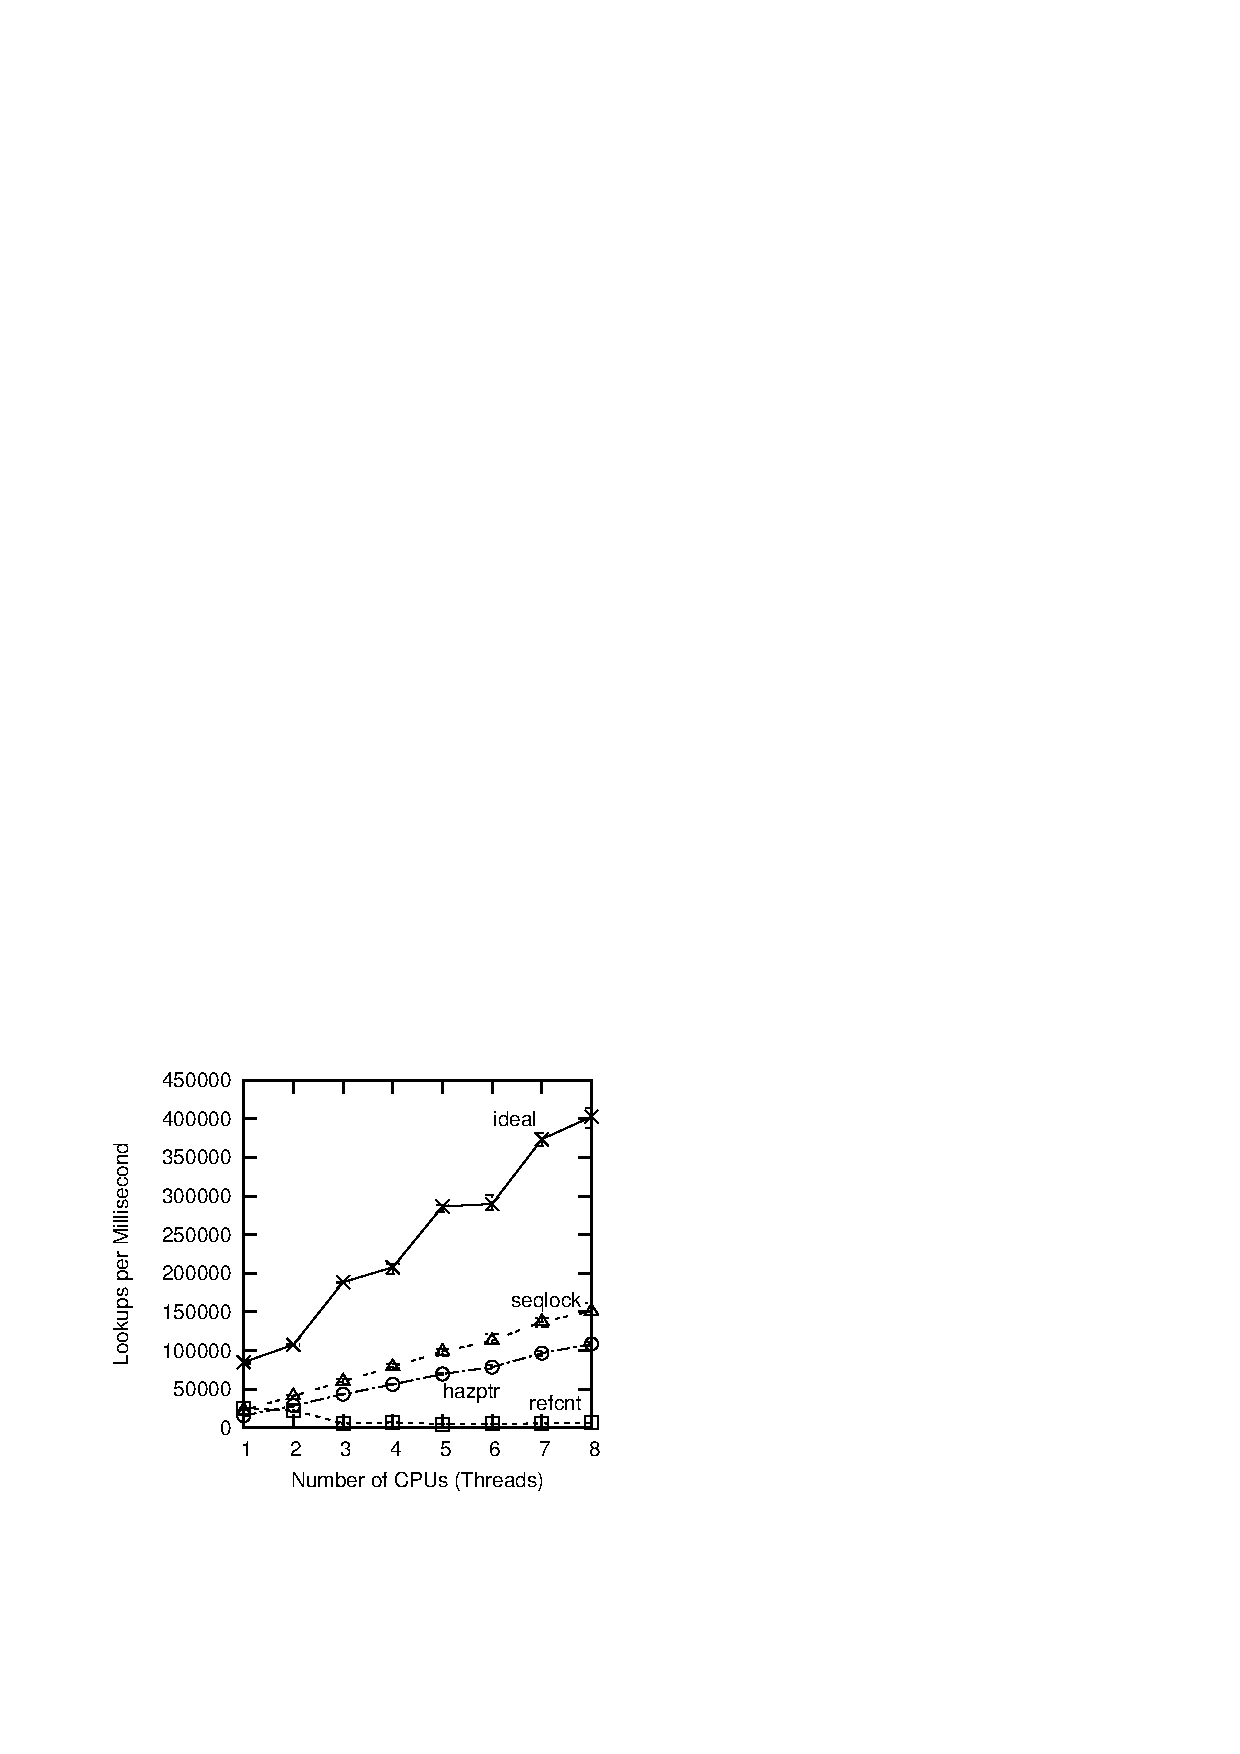
\includegraphics{CodeSamples/defer/perf-seqlock}}
\caption{Pre-BSD Routing Table Protected by Sequence Locking}
\label{fig:defer:Pre-BSD Routing Table Protected by Sequence Locking}
\end{figure}

Figure~\ref{fig:defer:Pre-BSD Routing Table Protected by Sequence Locking} 에서 볼 수 있듯이,
이 구현은 또한 read-only 워크로드에서 상당히 좋은 성능을 보입니다, 이상적인 성능에 비하면 여전히 멀었지만요.

안타깝지만, 이 구현 역시 해제 후 사용 문제를 가지고 있습니다.
문제는 읽기 쓰레드가 \co{read_seqretry()} 를 하기 전에 이미 해제된 구조체에
접근할 수 있기 때문에 segmentation violation 을 낼 수 있다는 점입니다.
\iffalse

It also performs better on the read-only workload, as can be seen in
Figure~\ref{fig:defer:Pre-BSD Routing Table Protected by Sequence Locking},
though its performance is still far from ideal.

Unfortunately, it also suffers use-after-free failures.
The problem is that the reader might encounter a segmentation violation
due to accessing an already-freed structure before it comes to the
\co{read_seqretry()}.
\fi

\QuickQuiz{}
	이 버그는 고쳐질 수 있을까요?
	달리 말해서, 동시의 삽입, 삭제, 탐색을 지원하는 링크드 리스트를
	보호하는 동기화 메커니즘으로 시퀀스락 \emph{하나만} 사용할 수 있을까요?
	\iffalse

	Can this bug be fixed?
	In other words, can you use sequence locks as the \emph{only}
	synchronization mechanism protecting a linked list supporting
	concurrent addition, deletion, and lookup?
	\fi
\QuickQuizAnswer{
	이를 가능하게 하는 한가지 방법은 read-only 액세스를 포함해 모든
	액세스들을 \co{write_seqlock()} 과 \co{write_sequnlock()} 으로
	감싸버리는 것입니다.
	물론, 이 방법은 모든 read-side 병렬성을 없애버릴 것이고, 커다란 락
	컨텐션을 초래하며, 더 나아가서 간단한 락킹처럼 쉽게 구현될 수 있을
	겁니다.

	Read-side 액세스를 보호하는데 \co{read_seqbegin()} 과
	\co{read_seqretry()} 를 사용하는 방법을 찾아낸다면, 그 방법이 다음의
	이벤트 시퀀스도 잘 처리할 수 있는지 확인해 보시기 바랍니다:
	\iffalse

	One trivial way of accomplishing this is to surround all
	accesses, including the read-only accesses, with
	\co{write_seqlock()} and \co{write_sequnlock()}.
	Of course, this solution also prohibits all read-side
	parallelism, resulting in massive lock contention,
	and furthermore could just as easily be implemented
	using simple locking.

	If you do come up with a solution that uses \co{read_seqbegin()}
	and \co{read_seqretry()} to protect read-side accesses, make
	sure that you correctly handle the following sequence of events:
	\fi

	\begin{enumerate}
	\item	CPU~0 가 링크드 리스트를 순회하고, 리스트 원소~A 로의 포인터를
		집어냅니다.
	\item	CPU~1 이 원소~A 를 리스트에서 제거하고 해제합니다.
	\item	CPU~2 가 관계없는 데이터 구조체를 하나 할당하는데, 이 과정에서
		원소~A 가 사용하고 있던 메모리를 받아오게 됩니다.
		원소~A 의 \co{->next} 포인터를 저장하는데 사용되던 영역은 이제
		이 관계없는 데이터 구조 내에서 floating-point 수를 저장하는데
		사용됩니다.
	\item	CPU~0 가 원소~A 의 \co{->next} 포인터였던 것을 보게 되는데,
		무작위적인 비트를 보게 되고, 따라서 segmentation fault 가 날
		겁니다.
	\iffalse

	\item	CPU~0 is traversing the linked list, and picks up a pointer
		to list element~A.
	\item	CPU~1 removes element~A from the list and frees it.
	\item	CPU~2 allocates an unrelated data structure, and gets
		the memory formerly occupied by element~A.
		In this unrelated data structure, the memory previously
		used for element~A's \co{->next} pointer is now occupied
		by a floating-point number.
	\item	CPU~0 picks up what used to be element~A's \co{->next}
		pointer, gets random bits, and therefore gets a
		segmentation fault.
	\fi
	\end{enumerate}

	이런 종류의 문제를 해결하기 위해서는 ``타입-안전 메모리'' 가 필요한데,
	이에 대해서는
	Section~\ref{sec:defer:RCU is a Way of Providing Type-Safe Memory} 에서
	다루도록 하겠습니다.
	하지만 이 경우, 시퀀스 락에 더해서 또다른 동기화 메커니즘을 사용해야
	할겁니다!
	\iffalse

	One way to protect against this sort of problem requires use
	of ``type-safe memory'', which will be discussed in
	Section~\ref{sec:defer:RCU is a Way of Providing Type-Safe Memory}.
	But in that case, you would be using some other synchronization
	mechanism in addition to sequence locks!
	\fi
} \QuickQuizEnd

시퀀스 락의 read-side 크리티컬 섹션도, write-side 크리티컬 섹션도 트랜잭션으로
생각될 수 있고, 따라서 시퀀스 락킹은 제한적인 형태의 트랜잭셔널 메모리로 생각될
수 있겠는데, 트랜잭셔널 메모리에 대해서는
Section~\ref{sec:future:Transactional Memory} 에서 이야기 하겠습니다.
시퀀스 락킹의 제약점들은: (1)~시퀀스 락킹은 업데이트를 제약하고 (2)~시퀀스
락킹은 업데이트 쓰레드에 의해 해제되었을 수 있는 오브젝트로의 포인터의 횡단을
허용하지 않습니다.
이런 제약점들은 물론 트랜잭셔널 메모리를 사용해 극복될 수 있습니다만, 다른
동기화 도구들을 시퀀스 락킹과 함께 사용해서도 극복될 수 있습니다.
\iffalse

Both the read-side and write-side critical sections of a sequence lock
can be thought of as transactions, and sequence locking therefore
can be thought of as a limited form of transactional memory, which
will be discussed in Section~\ref{sec:future:Transactional Memory}.
The limitations of sequence locking are: (1)~Sequence locking restricts
updates and (2)~sequence locking does not permit traversal of pointers
to objects that might be freed by updaters.
These limitations are of course overcome by transactional memory, but
can also be overcome by combining other synchronization primitives
with sequence locking.
\fi

시퀀스 락들은 쓰기를 하는 쓰레드들이 읽기를 하는 쓰레드들을 뒤로 미뤄지도록 할
수 있지만, 그 반대는 불가능합니다.
이는 공정하지 않고 쓰기가 대부분인 워크로드에서는 스타베이션을 낼수도
있습니다.
반면, 쓰기 쓰레드가 없다면, 시퀀스 락을 사용하는 읽기 쓰레드들은 합리적인
수준으로 빠르고 선형적으로 확장이 가능할 것입니다.
두가지 모두 최선인 경우를 원하는 게 사람입니다: 읽는 쪽의 실패나 스타베이션의
가능성 없는 빠른 읽기.
또한, 포인터들에 대한 제약점들 역시 극복된다면 좋을 겁니다.
다음 섹션은 이런 속성을 가진 동기화 메커니즘을 소개합니다.
\iffalse

Sequence locks allow writers to defer readers, but not vice versa.
This can result in unfairness and even starvation
in writer-heavy workloads.
On the other hand, in the absence of writers, sequence-lock readers are
reasonably fast and scale linearly.
It is only human to want the best of both worlds: fast readers without
the possibility of read-side failure, let alone starvation.
In addition, it would also be nice to overcome sequence locking's limitations
with pointers.
The following section presents a synchronization mechanism with exactly
these properties.
\fi
